\documentclass[12pt,a4paper]{article}
\usepackage[utf8]{inputenc}
\usepackage[english]{babel}
\usepackage{amsmath}
\usepackage{amsfonts}
\usepackage{amssymb}
\usepackage{graphicx}
\usepackage{tikz}
\usepackage{pgfplots}
\usepackage{geometry}
\usepackage{xcolor}
\usepackage{listings}
\usepackage{float}
\usepackage{subcaption}
\usepackage{hyperref}
\usepackage{fancyhdr}

% Page setup
\geometry{margin=1in}
\pagestyle{fancy}
\fancyhf{}
\rhead{TaskWeight Integration Architecture}
\lhead{2025}
\cfoot{\thepage}

% TikZ libraries
\usetikzlibrary{shapes,arrows,positioning,fit,backgrounds,decorations.pathreplacing}
\pgfplotsset{compat=1.18}

% Color definitions
\definecolor{primaryblue}{RGB}{33, 150, 243}
\definecolor{secondarygreen}{RGB}{76, 175, 80}
\definecolor{accentorange}{RGB}{255, 152, 0}
\definecolor{backgroundgray}{RGB}{245, 245, 245}
\definecolor{darkgray}{RGB}{66, 66, 66}

% Code listing setup
\lstset{
    backgroundcolor=\color{backgroundgray},
    basicstyle=\ttfamily\small,
    keywordstyle=\color{primaryblue}\bfseries,
    commentstyle=\color{darkgray},
    stringstyle=\color{secondarygreen},
    numbers=left,
    numberstyle=\tiny\color{darkgray},
    stepnumber=1,
    numbersep=5pt,
    frame=single,
    rulecolor=\color{darkgray},
    breaklines=true,
    showstringspaces=false,
    tabsize=2
}

\title{\textbf{TaskWeight Integration Architecture:\\A Revolutionary Approach to Software Development Estimation}}
\author{TaskWeight Development Team}
\date{2025}

\begin{document}

\maketitle

\section{Integration Architecture Overview}

TaskWeight's integration architecture represents a paradigm shift toward seamless workflow integration, leveraging cutting-edge technologies to create an intelligent, adaptive system that transforms how software development teams approach task estimation.

\subsection{High-Level System Architecture}

The TaskWeight ecosystem operates through a sophisticated multi-tier architecture designed for scalability, reliability, and seamless integration with existing development workflows.

\begin{figure}[H]
\centering
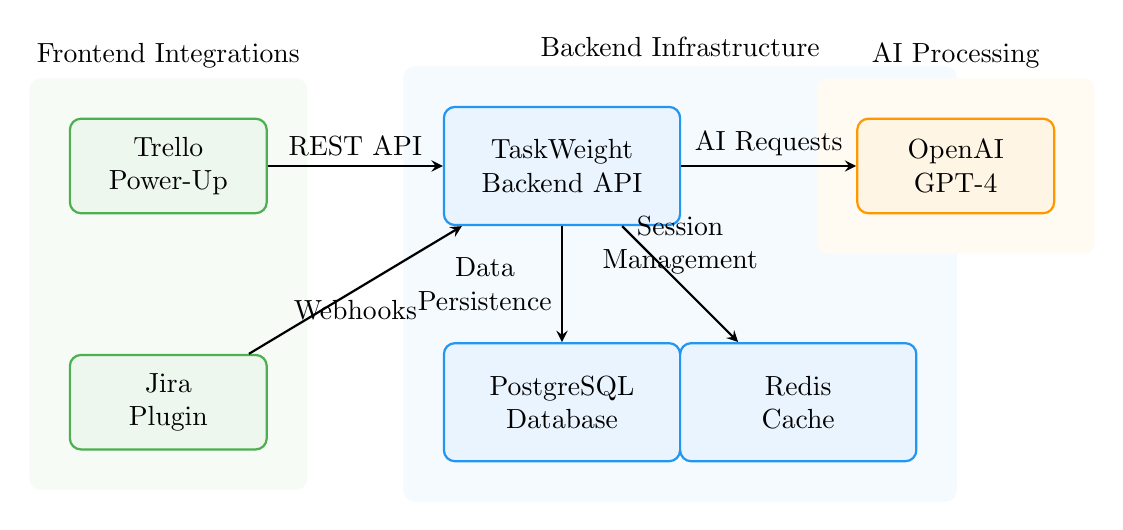
\begin{tikzpicture}[
    node distance=3cm,
    every node/.style={align=center},
    component/.style={rectangle, rounded corners, minimum width=3cm, minimum height=1.5cm, text centered, draw=primaryblue, fill=primaryblue!10, thick},
    plugin/.style={rectangle, rounded corners, minimum width=2.5cm, minimum height=1.2cm, text centered, draw=secondarygreen, fill=secondarygreen!10, thick},
    ai/.style={rectangle, rounded corners, minimum width=2.5cm, minimum height=1.2cm, text centered, draw=accentorange, fill=accentorange!10, thick},
    arrow/.style={thick,->,>=stealth}
]

% Main components
\node[plugin] (trello) {Trello\\Power-Up};
\node[plugin, below of=trello] (jira) {Jira\\Plugin};
\node[component, right of=trello, xshift=2cm] (api) {TaskWeight\\Backend API};
\node[ai, right of=api, xshift=2cm] (openai) {OpenAI\\GPT-4};
\node[component, below of=api] (db) {PostgreSQL\\Database};
\node[component, right of=db] (redis) {Redis\\Cache};

% Connections
\draw[arrow] (trello) -- (api) node[midway, above] {REST API};
\draw[arrow] (jira) -- (api) node[midway, below] {Webhooks};
\draw[arrow] (api) -- (openai) node[midway, above] {AI Requests};
\draw[arrow] (api) -- (db) node[midway, left] {Data\\Persistence};
\draw[arrow] (api) -- (redis) node[midway, above] {Session\\Management};

% Background
\begin{scope}[on background layer]
\node[fit=(trello)(jira), fill=secondarygreen!5, rounded corners, inner sep=0.5cm, label=above:Frontend Integrations] {};
\node[fit=(api)(db)(redis), fill=primaryblue!5, rounded corners, inner sep=0.5cm, label=above:Backend Infrastructure] {};
\node[fit=(openai), fill=accentorange!5, rounded corners, inner sep=0.5cm, label=above:AI Processing] {};
\end{scope}

\end{tikzpicture}
\caption{TaskWeight High-Level Architecture}
\label{fig:high-level-arch}
\end{figure}

\subsection{Component Interaction Flow}

The system operates through a sophisticated request-response cycle that ensures optimal performance and user experience:

\begin{figure}[H]
\centering
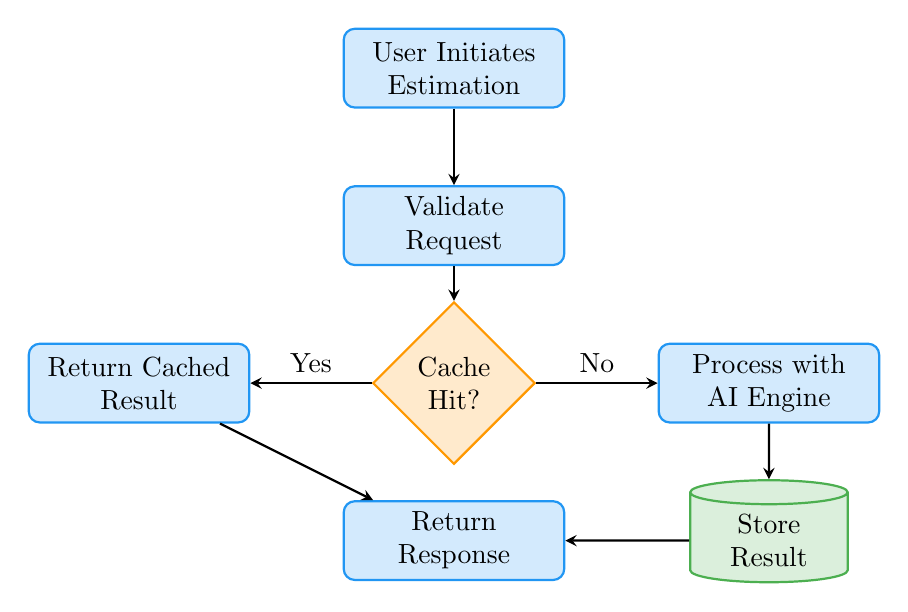
\begin{tikzpicture}[
    node distance=2cm,
    every node/.style={align=center},
    process/.style={rectangle, rounded corners, minimum width=2.8cm, minimum height=1cm, text centered, draw=primaryblue, fill=primaryblue!20, thick},
    decision/.style={diamond, minimum width=2cm, minimum height=1cm, text centered, draw=accentorange, fill=accentorange!20, thick},
    storage/.style={cylinder, shape border rotate=90, aspect=0.25, minimum width=2cm, minimum height=1cm, text centered, draw=secondarygreen, fill=secondarygreen!20, thick},
    arrow/.style={thick,->,>=stealth}
]

% Process flow
\node[process] (start) {User Initiates\\Estimation};
\node[process, below of=start] (validate) {Validate\\Request};
\node[decision, below of=validate] (cached) {Cache\\Hit?};
\node[process, left of=cached, xshift=-2cm] (return_cache) {Return Cached\\Result};
\node[process, right of=cached, xshift=2cm] (ai_process) {Process with\\AI Engine};
\node[storage, below of=ai_process] (store) {Store\\Result};
\node[process, below of=cached] (response) {Return\\Response};

% Arrows
\draw[arrow] (start) -- (validate);
\draw[arrow] (validate) -- (cached);
\draw[arrow] (cached) -- (return_cache) node[midway, above] {Yes};
\draw[arrow] (cached) -- (ai_process) node[midway, above] {No};
\draw[arrow] (return_cache) -- (response);
\draw[arrow] (ai_process) -- (store);
\draw[arrow] (store) -- (response);

\end{tikzpicture}
\caption{TaskWeight Processing Flow}
\label{fig:processing-flow}
\end{figure}

\section{Real-time Integration Components}

\subsection{Trello Power-Up Integration}

The Trello Power-Up represents a seamless integration that transforms traditional project management into an AI-powered estimation platform.

\begin{figure}[H]
\centering
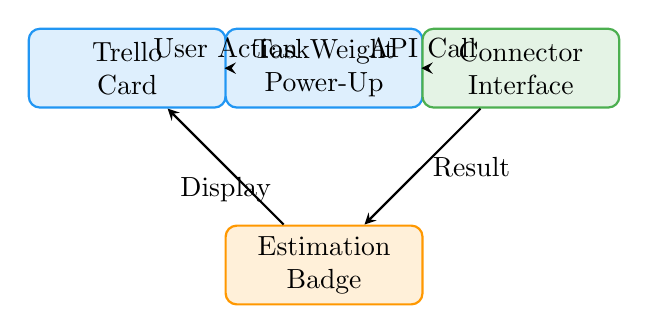
\begin{tikzpicture}[
    node distance=2.5cm,
    every node/.style={align=center},
    ui/.style={rectangle, rounded corners, minimum width=2.5cm, minimum height=1cm, text centered, draw=primaryblue, fill=primaryblue!15, thick},
    api/.style={rectangle, rounded corners, minimum width=2.5cm, minimum height=1cm, text centered, draw=secondarygreen, fill=secondarygreen!15, thick},
    data/.style={rectangle, rounded corners, minimum width=2.5cm, minimum height=1cm, text centered, draw=accentorange, fill=accentorange!15, thick},
    arrow/.style={thick,->,>=stealth}
]

% Trello integration components
\node[ui] (card) {Trello\\Card};
\node[ui, right of=card] (powerup) {TaskWeight\\Power-Up};
\node[api, right of=powerup] (connector) {Connector\\Interface};
\node[data, below of=powerup] (estimation) {Estimation\\Badge};

% Connections
\draw[arrow] (card) -- (powerup) node[midway, above] {User Action};
\draw[arrow] (powerup) -- (connector) node[midway, above] {API Call};
\draw[arrow] (connector) -- (estimation) node[midway, right] {Result};
\draw[arrow] (estimation) -- (card) node[midway, below] {Display};

\end{tikzpicture}
\caption{Trello Power-Up Integration Flow}
\label{fig:trello-integration}
\end{figure}

\subsection{Jira Plugin Architecture}

The Jira plugin provides enterprise-grade integration with advanced workflow management capabilities.

\begin{lstlisting}[language=JavaScript, caption=Jira Plugin Configuration]
// Jira Plugin Manifest
{
  "key": "taskweight-jira-plugin",
  "name": "TaskWeight Estimation Plugin",
  "description": "AI-powered task estimation for Jira",
  "vendor": {
    "name": "TaskWeight Team",
    "url": "https://taskweight.ai"
  },
  "baseUrl": "https://api.taskweight.ai/jira",
  "authentication": {
    "type": "jwt"
  },
  "scopes": [
    "READ",
    "WRITE",
    "PROJECT_ADMIN"
  ],
  "modules": {
    "webPanels": [
      {
        "key": "taskweight-panel",
        "location": "atl.jira.view.issue.right.context",
        "url": "/panel/estimation?issueKey={issue.key}"
      }
    ],
    "webSections": [
      {
        "key": "taskweight-section",
        "location": "atl.jira.view.issue.right.context"
      }
    ]
  }
}
\end{lstlisting}

\section{Asynchronous Processing Architecture}

TaskWeight implements a sophisticated asynchronous processing system that ensures optimal performance and scalability.

\subsection{Queue Management System}

\begin{figure}[H]
\centering
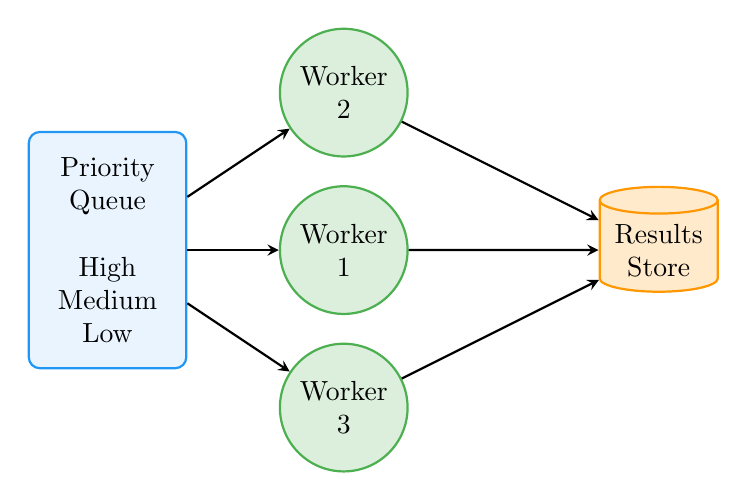
\begin{tikzpicture}[
    node distance=2cm,
    every node/.style={align=center},
    queue/.style={rectangle, rounded corners, minimum width=2cm, minimum height=3cm, text centered, draw=primaryblue, fill=primaryblue!10, thick},
    worker/.style={circle, minimum width=1.5cm, text centered, draw=secondarygreen, fill=secondarygreen!20, thick},
    storage/.style={cylinder, shape border rotate=90, aspect=0.25, minimum width=1.5cm, minimum height=1cm, text centered, draw=accentorange, fill=accentorange!20, thick},
    arrow/.style={thick,->,>=stealth}
]

% Queue system
\node[queue] (priority_queue) {Priority\\Queue\\\\High\\Medium\\Low};
\node[worker, right of=priority_queue, xshift=1cm] (worker1) {Worker\\1};
\node[worker, above of=worker1] (worker2) {Worker\\2};
\node[worker, below of=worker1] (worker3) {Worker\\3};
\node[storage, right of=worker1, xshift=2cm] (results) {Results\\Store};

% Connections
\draw[arrow] (priority_queue) -- (worker1);
\draw[arrow] (priority_queue) -- (worker2);
\draw[arrow] (priority_queue) -- (worker3);
\draw[arrow] (worker1) -- (results);
\draw[arrow] (worker2) -- (results);
\draw[arrow] (worker3) -- (results);

\end{tikzpicture}
\caption{Asynchronous Processing Queue System}
\label{fig:queue-system}
\end{figure}

\subsection{AI Processing Pipeline}

The AI processing pipeline represents the core innovation of TaskWeight, transforming raw task descriptions into precise, actionable estimates.

\begin{lstlisting}[language=Python, caption=Asynchronous Task Processing]
import asyncio
from typing import Optional
from dataclasses import dataclass

@dataclass
class EstimationRequest:
    card_id: str
    task_description: str
    repo_url: str
    priority: str = "medium"
    complexity: str = "medium"
    user_id: Optional[str] = None

class AsyncTaskProcessor:
    def __init__(self, storage, ai_client):
        self.storage = storage
        self.ai_client = ai_client
        self.processing_queue = asyncio.Queue()
        
    async def estimate_task(self, request: EstimationRequest):
        """Asynchronously processes task estimation"""
        # Create initial estimation record
        estimation = await self.storage.create_estimation(
            request.card_id, 
            request.user_id,
            status="processing"
        )
        
        try:
            # Generate AI-powered estimation
            prompt = self._create_estimation_prompt(request)
            
            # Process through OpenAI API with retry logic
            response = await self._process_with_retry(prompt)
            
            # Parse and validate response
            parsed_result = self._parse_ai_response(response)
            
            # Update estimation with results
            await self.storage.update_estimation(
                estimation.id,
                estimated_hours=parsed_result.hours,
                confidence_score=parsed_result.confidence,
                reasoning=parsed_result.reasoning,
                breakdown=parsed_result.breakdown,
                status="completed"
            )
            
            return estimation
            
        except Exception as e:
            await self.storage.update_estimation(
                estimation.id,
                status="failed",
                error_message=str(e)
            )
            raise
            
    async def _process_with_retry(self, prompt, max_retries=3):
        """Process AI request with exponential backoff"""
        for attempt in range(max_retries):
            try:
                response = await self.ai_client.chat.completions.create(
                    model="gpt-4",
                    messages=[{"role": "user", "content": prompt}],
                    temperature=0.1,
                    max_tokens=1000
                )
                return response
            except Exception as e:
                if attempt == max_retries - 1:
                    raise
                await asyncio.sleep(2 ** attempt)
\end{lstlisting}

\section{Data Intelligence Layer}

\subsection{Performance Metrics Architecture}

TaskWeight implements a comprehensive performance tracking system that enables continuous improvement and personalized estimations.

\begin{figure}[H]
\centering
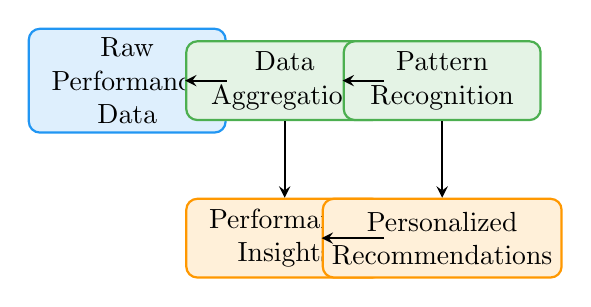
\begin{tikzpicture}[
    node distance=2cm,
    every node/.style={align=center},
    metric/.style={rectangle, rounded corners, minimum width=2.5cm, minimum height=1cm, text centered, draw=primaryblue, fill=primaryblue!15, thick},
    analysis/.style={rectangle, rounded corners, minimum width=2.5cm, minimum height=1cm, text centered, draw=secondarygreen, fill=secondarygreen!15, thick},
    output/.style={rectangle, rounded corners, minimum width=2.5cm, minimum height=1cm, text centered, draw=accentorange, fill=accentorange!15, thick},
    arrow/.style={thick,->,>=stealth}
]

% Metrics flow
\node[metric] (raw_data) {Raw\\Performance\\Data};
\node[analysis, right of=raw_data] (aggregation) {Data\\Aggregation};
\node[analysis, right of=aggregation] (pattern) {Pattern\\Recognition};
\node[output, below of=aggregation] (insights) {Performance\\Insights};
\node[output, right of=insights] (recommendations) {Personalized\\Recommendations};

% Connections
\draw[arrow] (raw_data) -- (aggregation);
\draw[arrow] (aggregation) -- (pattern);
\draw[arrow] (aggregation) -- (insights);
\draw[arrow] (pattern) -- (recommendations);
\draw[arrow] (insights) -- (recommendations);

\end{tikzpicture}
\caption{Performance Metrics Processing Pipeline}
\label{fig:metrics-pipeline}
\end{figure}

\subsection{Database Schema Optimization}

The TaskWeight database schema is optimized for high-performance analytics and real-time querying.

\begin{lstlisting}[language=SQL, caption=Optimized Database Views]
-- High-Performance Estimation Analytics View
CREATE MATERIALIZED VIEW estimation_analytics AS
SELECT 
    er.user_id,
    er.project_id,
    er.complexity,
    er.priority,
    AVG(er.estimated_hours) as avg_estimated_hours,
    AVG(ef.actual_hours) as avg_actual_hours,
    AVG(ef.accuracy) as avg_accuracy,
    COUNT(*) as total_estimations,
    STDDEV(ef.accuracy) as accuracy_variance,
    DATE_TRUNC('week', er.created_at) as estimation_week
FROM estimation_results er
LEFT JOIN estimation_feedback ef ON er.id = ef.estimation_id
WHERE er.status = 'completed'
  AND ef.actual_hours IS NOT NULL
GROUP BY 
    er.user_id, 
    er.project_id, 
    er.complexity, 
    er.priority,
    DATE_TRUNC('week', er.created_at)
WITH DATA;

-- Refresh strategy for real-time analytics
CREATE UNIQUE INDEX ON estimation_analytics 
    (user_id, project_id, complexity, priority, estimation_week);

-- Automated refresh trigger
CREATE OR REPLACE FUNCTION refresh_estimation_analytics()
RETURNS TRIGGER AS $$
BEGIN
    REFRESH MATERIALIZED VIEW CONCURRENTLY estimation_analytics;
    RETURN NULL;
END;
$$ LANGUAGE plpgsql;

CREATE TRIGGER estimation_analytics_refresh
    AFTER INSERT OR UPDATE OR DELETE ON estimation_feedback
    FOR EACH STATEMENT
    EXECUTE FUNCTION refresh_estimation_analytics();
\end{lstlisting}

\section{Security and Scalability Architecture}

\subsection{Security Framework}

TaskWeight implements enterprise-grade security measures to protect sensitive project data and maintain user privacy.

\begin{figure}[H]
\centering
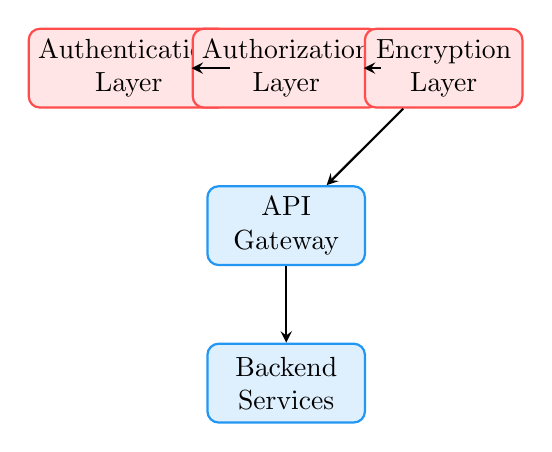
\begin{tikzpicture}[
    node distance=2cm,
    every node/.style={align=center},
    security/.style={rectangle, rounded corners, minimum width=2cm, minimum height=1cm, text centered, draw=red!70, fill=red!10, thick},
    process/.style={rectangle, rounded corners, minimum width=2cm, minimum height=1cm, text centered, draw=primaryblue, fill=primaryblue!15, thick},
    arrow/.style={thick,->,>=stealth}
]

% Security layers
\node[security] (auth) {Authentication\\Layer};
\node[security, right of=auth] (authz) {Authorization\\Layer};
\node[security, right of=authz] (encryption) {Encryption\\Layer};
\node[process, below of=authz] (api) {API\\Gateway};
\node[process, below of=api] (backend) {Backend\\Services};

% Connections
\draw[arrow] (auth) -- (authz);
\draw[arrow] (authz) -- (encryption);
\draw[arrow] (encryption) -- (api);
\draw[arrow] (api) -- (backend);

\end{tikzpicture}
\caption{Security Architecture Layers}
\label{fig:security-arch}
\end{figure}

\subsection{Horizontal Scaling Strategy}

TaskWeight's architecture supports horizontal scaling to accommodate growing user bases and increasing estimation volumes.

\begin{figure}[H]
\centering
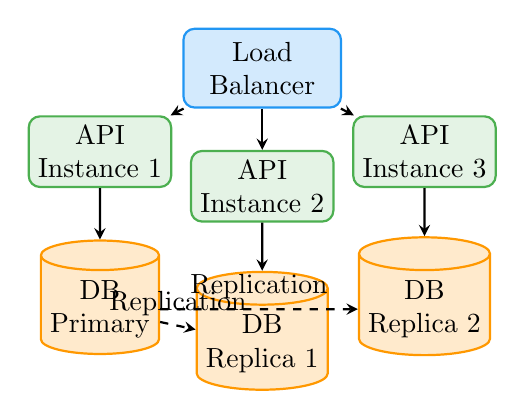
\begin{tikzpicture}[
    node distance=1.5cm,
    every node/.style={align=center},
    lb/.style={rectangle, rounded corners, minimum width=2cm, minimum height=1cm, text centered, draw=primaryblue, fill=primaryblue!20, thick},
    service/.style={rectangle, rounded corners, minimum width=1.5cm, minimum height=0.8cm, text centered, draw=secondarygreen, fill=secondarygreen!15, thick},
    db/.style={cylinder, shape border rotate=90, aspect=0.25, minimum width=1.5cm, minimum height=0.8cm, text centered, draw=accentorange, fill=accentorange!20, thick},
    arrow/.style={thick,->,>=stealth}
]

% Load balancer
\node[lb] (lb) {Load\\Balancer};

% Service instances
\node[service, below left of=lb, xshift=-1cm] (service1) {API\\Instance 1};
\node[service, below of=lb] (service2) {API\\Instance 2};
\node[service, below right of=lb, xshift=1cm] (service3) {API\\Instance 3};

% Database cluster
\node[db, below of=service1, yshift=-0.5cm] (db1) {DB\\Primary};
\node[db, below of=service2, yshift=-0.5cm] (db2) {DB\\Replica 1};
\node[db, below of=service3, yshift=-0.5cm] (db3) {DB\\Replica 2};

% Connections
\draw[arrow] (lb) -- (service1);
\draw[arrow] (lb) -- (service2);
\draw[arrow] (lb) -- (service3);
\draw[arrow] (service1) -- (db1);
\draw[arrow] (service2) -- (db2);
\draw[arrow] (service3) -- (db3);

% Replication arrows
\draw[arrow, dashed] (db1) -- (db2) node[midway, above] {Replication};
\draw[arrow, dashed] (db1) -- (db3) node[midway, above] {Replication};

\end{tikzpicture}
\caption{Horizontal Scaling Architecture}
\label{fig:scaling-arch}
\end{figure}

\section{Conclusion}

TaskWeight's integration architecture represents a revolutionary approach to software development estimation, combining cutting-edge AI technology with robust, scalable infrastructure. The system's modular design ensures seamless integration with existing workflows while providing the flexibility to adapt to evolving development practices.

The architecture's emphasis on asynchronous processing, intelligent caching, and comprehensive performance tracking creates a foundation for continuous improvement and personalized estimation experiences. As software development continues to evolve, TaskWeight's architecture positions teams to leverage AI-driven insights for more accurate, efficient, and predictable project delivery.

Through its sophisticated integration capabilities, TaskWeight transforms traditional project management tools into intelligent estimation platforms, ushering in a new era of data-driven software development planning.

\end{document}
